\documentclass{beamer}
\setbeamertemplate{footline}[page number]
\date{}
\author{}
\institute{}

%%%%%%% Put these names back in the final version 
%\\Aswathy Rajendra Kurup\\Meenu Ajith}
%\institute{Department of Electrical and Computer Engineering\\The University of New Mexico}
\setbeamercovered{transparent}
\usepackage{setspace}
\usepackage{array}
\usepackage[T1]{fontenc}
\usepackage{graphicx}
\usepackage{amsmath}
\usepackage{amsfonts}
\usepackage{amssymb}
\usepackage{makeidx}
\usefonttheme{serif}
\usepackage{multirow}
\usepackage{booktabs} 
\usepackage{rotating}
\usepackage{color}
\usepackage{float}
\usepackage[latin1]{inputenc}
\usepackage[english]{babel}
\usepackage{amsmath}
\usepackage{amsfonts}
\usepackage{eurosym}
\usepackage{rotating}
\usepackage{multicol}
\usepackage{pythonhighlight}
\usepackage[normalem]{ulem}
\newcommand{\ba}{{\bf a}}
\newcommand{\bb}{{\bf b}}
\newcommand{\bc}{{\bf c}}
\newcommand{\bd}{{\bf d}}
\newcommand{\be}{{\bf e}}
\newcommand{\bbf}{{\bf f}}
\newcommand{\bg}{{\bf g}}
\newcommand{\bh}{{\bf h}}
\newcommand{\bi}{{\bf i}}
\newcommand{\bk}{{\bf k}}
\newcommand{\bl}{{\bf l}}
\newcommand{\bm}{{\bf m}}
\newcommand{\bn}{{\bf n}}
\newcommand{\bo}{{\bf o}}
\newcommand{\bp}{{\bf p}}
\newcommand{\bq}{{\bf q}}
\newcommand{\br}{{\bf r}}
\newcommand{\bs}{{\bf s}}
\newcommand{\bt}{{\bf t}}
\newcommand{\bu}{{\bf u}}
\newcommand{\bv}{{\bf v}}
\newcommand{\bw}{{\bf w}}
\newcommand{\bx}{{\bf x}}
\newcommand{\by}{{\bf y}}
\newcommand{\bz}{{\bf z}}

\newcommand{\bA}{{\bf A}}
\newcommand{\bB}{{\bf B}}
\newcommand{\bC}{{\bf C}}
\newcommand{\bE}{{\bf E}}
\newcommand{\bG}{{\bf G}}
\newcommand{\bH}{{\bf H}}
\newcommand{\bI}{{\bf I}}
\newcommand{\bK}{{\bf K}}
\newcommand{\bL}{{\bf L}}
\newcommand{\bM}{{\bf M}}
\newcommand{\bO}{{\bf O}}
\newcommand{\bQ}{{\bf Q}}
\newcommand{\bR}{{\bf R}}
\newcommand{\bS}{{\bf S}}
\newcommand{\bT}{{\bf T}}
\newcommand{\bV}{{\bf V}}
\newcommand{\bW}{{\bf W}}
\newcommand{\bX}{{\bf X}}
\newcommand{\bY}{{\bf Y}}
\newcommand{\bZ}{{\bf Z}}
\newcommand\uptocnt{\stackrel{\mathclap{\normalfont\mbox{c}}}{\propto}}
\newcommand{\bpt}{{\bf pt}}
\newcommand{\bpl}{{\bf pl}}
\newcommand{\bdp}{{\bf dp}}
\newcommand{\btemp}{{\bf temp}}

\newcommand{\bmu}{{\boldsymbol \mu}}
\newcommand{\bSigma}{{\boldsymbol \Sigma}}
\newcommand{\bsigma}{{\boldsymbol \sigma}}
\newcommand{\bvarPhi}{{\boldsymbol \varPhi}}
\newcommand{\bvarphi}{{\boldsymbol \varphi}}
\newcommand{\bPhi}{{\boldsymbol \Phi}}
\newcommand{\bdelta}{{\boldsymbol \delta}}
\newcommand{\bZero}{{\bf 0}}
\newcommand{\bOne}{{\bf 1}}
\newcommand{\balpha}{{\boldsymbol \alpha}}
\newcommand{\bAlpha}{{\boldsymbol A}}
\newcommand{\btheta}{{\boldsymbol \theta}}

\newcommand{\softmax}{\text{softmax}}
\newcommand{\diag}{\text{diag}}
\newcommand{\sinc}{\mathrm{sinc}}
\newcommand{\argmin}{\mathop{\mathrm{argmin}}}
\newcommand{\infl}{\eta}
\newcommand{\Ind}{\mathrm{I}}
\newcommand{\Real}{\mathbb R}
\newcommand{\Intg}{\mathbb Z}
\newcommand{\Complex}{\mathbb C}
\newcommand{\Natural}{\mathbb N}
\newcommand{\Fourier}[1]{\mathcal{F} \{#1\}}
%\newcommand{\ii}{\mathbbm{i}}
\newcommand{\bphi}{\boldsymbol{\mathit{\phi}}}

\newcommand{\hs}{\hspace{2pt}}
\newcommand{\sign}{\text{sign}}
\author{Manel Mart\'inez-Ram\'on\\Meenu Ajith\\Aswathy Rajendra Kurup}

\usetheme{Madrid}
\usecolortheme{beaver}
\usepackage{tikz}
\usetikzlibrary{fit,arrows,calc,positioning}
\usepackage{listings}
\usepackage{xcolor}
\usepackage{emerald} 
\usepackage[T1]{fontenc} 
\usepackage{verbatim}
\usepackage{graphicx}
\usepackage{epsfig}
\usepackage{psfrag}
\usepackage[english]{babel}
\usepackage{listings}
\usepackage{courier}
\usepackage{color}
 \usepackage{vwcol} 
 \usepackage[english]{babel} % To obtain English text with the blindtext package
\usepackage{blindtext}
\definecolor{codegreen}{rgb}{0,0.6,0}
\definecolor{codegray}{rgb}{0.5,0.5,0.5}
\definecolor{codepurple}{rgb}{0.58,0,0.82}
\definecolor{backcolour}{rgb}{0.95,0.95,0.92}

\lstdefinestyle{mystyle}{
  backgroundcolor=\color{backcolour},   commentstyle=\color{codegreen},
  keywordstyle=\color{magenta},
  numberstyle=\tiny\color{codegray},
  stringstyle=\color{codepurple},
  basicstyle=\ttfamily\footnotesize,
  breakatwhitespace=false,         
  breaklines=true,                 
  captionpos=b,                    
  keepspaces=true,                 
  numbers=left,                    
  numbersep=5pt,                  
  showspaces=false,                
  showstringspaces=false,
  showtabs=false,                  
  tabsize=2
}
\lstset{style=mystyle}

%% Stuff for movies

% %\newcommand{\bt}{{\bf t}}
% \newcommand{\br}{{\bf r}}
% \newcommand{\bs}{{\bf s}}
% \newcommand{\by}{{\bf y}}
% \newcommand{\bz}{{\bf z}}
% \newcommand{\bx}{{\bf x}}
% \newcommand{\bw}{{\bf w}}
% \newcommand{\be}{{\bf e}}
% \newcommand{\bbf}{{\bf f}}
% \newcommand{\bb}{{\bf b}}
% \newcommand{\bd}{{\bf d}}
% \newcommand{\bA}{{\bf A}}
% \newcommand{\bB}{{\bf B}}
% \newcommand{\bL}{{\bf L}}
% \newcommand{\bM}{{\bf M}}

% \newcommand{\bC}{{\bf C}}
% \newcommand{\bI}{{\bf I}}
% \newcommand{\bK}{{\bf K}}
% \newcommand{\bk}{{\bf k}}
% \newcommand{\bT}{{\bf T}}
% \newcommand{\bV}{{\bf V}}
% \newcommand{\bW}{{\bf W}}
% \newcommand{\bX}{{\bf X}}
% \newcommand{\bY}{{\bf Y}}
% \newcommand{\bZ}{{\bf Z}}
% \newcommand{\bm}{{\bf m}}
% \newcommand{\bpt}{{\bf pt}}
% \newcommand{\bpl}{{\bf pl}}
% \newcommand{\bdp}{{\bf dp}}
% \newcommand{\btemp}{{\bf temp}}
% \newcommand{\bl}{{\bf l}}
% \newcommand{\bu}{{\bf u}}
% \newcommand{\bmu}{{\boldsymbol \mu}}
% \newcommand{\bSigma}{{\boldsymbol \Sigma}}
% \newcommand{\bLambda}{{\boldsymbol \Lambda}}

% \newcommand{\bsigma}{{\boldsymbol \sigma}}
% \newcommand{\bvarphi}{{\boldsymbol \varPhi}}
% \newcommand{\btheta}{{\boldsymbol \theta}}
% \newcommand{\bZero}{{\bf 0}}
% \newcommand{\balpha}{{\boldsymbol \alpha}}
% \newcommand{\bpi}{{\boldsymbol \pi}}
% \newcommand{\bxi}{{\boldsymbol \xi}}
% \newcommand{\bdelta}{{\boldsymbol \delta}}
\lstset{
	language=Python,
	basicstyle=\footnotesize\ttfamily\color{black},
	commentstyle = \footnotesize\ttfamily\color{red},
	keywordstyle=\footnotesize\ttfamily\color{blue},
	stringstyle=\footnotesize\ttfamily\color{black},
%	columns=fixed,
%	numbers=left,    
	numberstyle=\tiny,
	stepnumber=1,
	numbersep=5pt,
	tabsize=1,
	extendedchars=true,
	breaklines=true,            
	frame=b,         
	showspaces=false,
	showtabs=true,
	xleftmargin=6pt,
	framexleftmargin=6pt,
	framexrightmargin=2pt,
	framexbottommargin=4pt,
	showstringspaces=false      
}

\lstloadlanguages{
         Python
}

%\graphicspath{ {./images/} }  % Figures path - used in graphicx

%\selectcolormodel{cmyk}

\mode<presentation>

\newcommand{\dred}{darkred!90!black}
\newcommand{\written}{\ECFJD\textcolor{cyan!50!white}}
\newcommand{\hlight}{\textcolor{\dred}}
\newcommand{\Ex}{\textcolor{\dred}{Ex. }}

% remove navigation symbols in full screen mode
\setbeamertemplate{navigation symbols}{}  
\setbeamertemplate{blocks}[rounded][shadow=false]
\setbeamercolor{note page}{fg=black}

\setbeamercolor{title}{fg=\dred}
\setbeamercolor{frametitle}{fg=white}
\setbeamercolor{frametitle}{bg=\dred}
\setbeamercolor{structure}{fg=black,bg=white}
\setbeamercolor{background canvas}{bg=white,fg=black}
\setbeamercolor{normal text}{fg=black,bg=white}
\setbeamercolor{item}{fg=red!80!black,bg=white!}
\addtobeamertemplate{block begin}{\setbeamercolor{block title}{fg=white,bg=\dred}
\setbeamercolor{block body}{fg=white,bg=gray}}{}


\title{6. Attention-based networks}
\subtitle{6.2. Transformers}

\addtobeamertemplate{frametitle}{}


\begin{document}
\maketitle


\begin{frame}{Self-attention models}{Introduction}
\begin{itemize}
\item  A self-attention model is a mechanism where each token has its own query, keys and values.
\item Each token attends to each other token based on their key vectors. 
\item This constructs a representation of the sequence of tokens which is based on a weighted sum over the rest of the tokens.
\item This is also called an intra-attention model.

\end{itemize}
\end{frame}
\begin{frame}{Self-attention models}{Definitnion}
\begin{itemize}

\item Assume a sequence of input tokens $\bx_1, \cdots \bx_N$. A self-attention model outputs a sequence of $N$ vectors $\by_1, \cdots \, \by_N$ of the same dimension. 
    \item The equation of the model can be written as
\begin{equation}
    \mathbf{y}_i = f(\mathbf{x}_i, (\mathbf{x}_1, \mathbf{x}_1), \ldots, (\mathbf{x}_n, \mathbf{x}_n))
\end{equation}

\item This is a representation that is alternative to the RNN encoder-decoder seen in the previous lesson. 

\end{itemize}    
\end{frame}

\begin{frame}{Self-attention models}{Comparative complexities}

\begin{multicols}{2}
\begin{center}
\includegraphics[scale=0.6]{Module 6 (Attention-based networks)/pics/cnn-complexity.pdf}
\end{center}

\columnbreak
Convolutional neural network with kernels of size $k$.
\begin{itemize}
    \item Computational complexity: $\mathcal{O}(kND^2)$.
    \item Sequential operations: $\mathcal{O}(1)$.
    \item Maximum path length between tokens $\mathcal{O}(N/k)$. 
\end{itemize}

\end{multicols}
\end{frame}

\begin{frame}{Self-attention models}{Comparative complexities}

\begin{multicols}{2}
\begin{center}
\includegraphics[scale=0.6]{Module 6 (Attention-based networks)/pics/rnn-complexity.pdf}
\end{center}

\columnbreak
Recurrent neural networks.
\begin{itemize}
    \item Computational complexity of hidden state computation: $\mathcal{O}(ND^2)$.
    \item Sequential operations: $\mathcal{O}(n)$.
    \item Maximum path length between tokens $\mathcal{O}(N)$. 
\end{itemize}

\end{multicols}
\end{frame}

\begin{frame}{Self-attention models}{Comparative complexities}

\begin{multicols}{2}
\begin{center}
\includegraphics[scale=0.6]{Module 6 (Attention-based networks)/pics/self-attention-complexity.pdf}
\end{center}

\columnbreak
Self-attention models.
\begin{itemize}
    \item Computational complexity: $\mathcal{O}(N^2D)$.
    \item Sequential operations: $\mathcal{O}(1)$.
    \item Maximum path length between tokens $\mathcal{O}(1)$. 
\end{itemize}

\end{multicols}

CNN and self-attention have parallel computing properties. Self-attention has the shortest maximum path, but its $N^2$ is bad for long sequences 

\end{frame}

\begin{frame}{Positional encoding}
\begin{itemize}
    \item Self-attention avoids recurrent operation so parallel computing can be used.
    \item However, it does not pay \emph{attention} to the order of the sequence.
    \item We need a mechanism to explain how the sequence arrived. 
    \item This can be learned or fixed.
    \item The first positional encoding for transformers was the trigonometric positional encoding
    
\end{itemize}
    
\end{frame}

\begin{frame}{Positional encoding}
\begin{itemize}
\item Assume that the embeddings $\bx_1, \cdots, \bx_N$ for the $N$ tokens of a sequence are available.  
\item The positional encoding adds a vector $\bp_n$ to each embedding with elements
\begin{equation}
    \begin{split}\begin{aligned} p_{2j,n} &= \sin\left(\frac{n}{10000^{2j/D}}\right)\\p_{2j+1,n} &= \cos\left(\frac{n}{10000^{2j/D}}\right)\end{aligned}\end{split}
    \end{equation}
where the first expression corresponds to elements with index even of vector $\bp_n$ and the second to odd elements.
\item The coded vector is $\bx_n + \bp_n$
\end{itemize} 
\end{frame}
\begin{frame}{Positional encoding}
\begin{center}
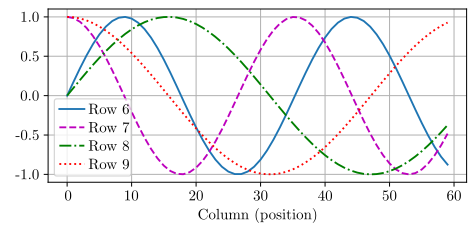
\includegraphics[scale=0.5]{Module 6 (Attention-based networks)/pics/output_self-attention-and-positional-encoding.pdf}
 \end{center}   
 This can be compared to the binary coding
% \usepackage{tabularray}
\begin{table}[]
\begin{tabular}{|l|llllllllllllllll|}
\hline
&\multicolumn{16}{|c|}{Position}                                     \\
\hline
A & 0 & 1 & 0 & 1 & 0 & 1 & 0 & 1 & 0 & 1 & 0 & 1 & 0 & 1 & 0 & 1 \\
B & 0 & 0 & 1 & 1 & 0 & 0 & 1 & 1 & 0 & 0 & 1 & 1 & 0 & 0 & 1 & 1 \\
C & 0 & 0 & 0 & 0 & 1 & 1 & 1 & 1 & 0 & 0 & 0 & 0 & 1 & 1 & 1 & 1\\
\hline
\end{tabular}
\end{table}
\end{frame}

\begin{frame}{The transformer}{Introduction}
\begin{itemize}
    \item Self-attention uses parallel computation and the shortest maximum path length.
    \item Deep structures for sequence encoding-decoding can be constructed with this strategy.
    \item The Transformer model is based only in self-attention mechanisms without CNN or RNN. 
    \item Transformers are used in language, vision, speech or reinforcement learning. 
\end{itemize}
\end{frame}

\begin{frame}{The transformer}{Overall structure}
\vspace{-0.8cm}
\begin{multicols}{2}
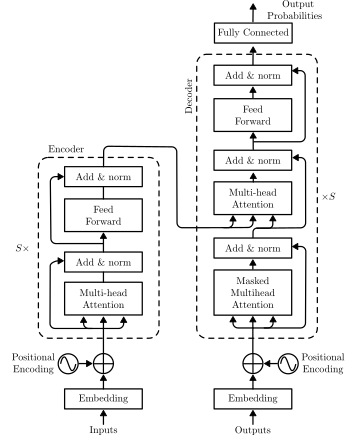
\includegraphics[scale=0.49]{Module 6 (Attention-based networks)/pics/transformer.pdf}
\columnbreak    


This is the overall structure of a transformer. 
\begin{itemize}
    \item The input and output sequences are added to a positional encoding.
    \item The encoder is a stack of identical layers.
    \item Each input is the output of the previous layer. 
    \item The add \& norm (residual) block adds the input and the output of the previous one, which has the same size.  
    \end{itemize}

\end{multicols}
\end{frame}



\begin{frame}{The transformer}{Overall structure}
\vspace{-0.8cm}
\begin{multicols}{2}
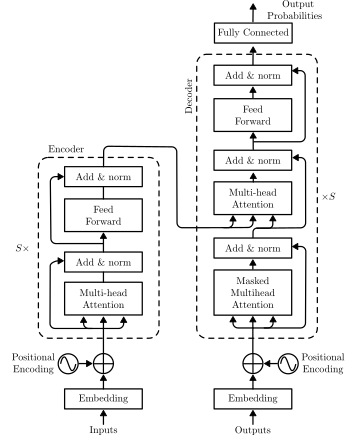
\includegraphics[scale=0.49]{Module 6 (Attention-based networks)/pics/transformer.pdf}
\columnbreak    
\begin{itemize}
    \item   The decoder is also a stack of multiple identical layers with residual and normalizations.
    \item The central sublayer inserts the encoder input as keys and values in a block called the encoder-decoder attention.
    \item The masked attention allows each position to attend to all positions until that position. 

    That prevents a position to attend subsequent positions.

    \item Originally, S=6.
\end{itemize}

\end{multicols}
\end{frame}
\begin{frame}{The transformer}{Basic operation}
    \begin{itemize}
        \item The transformer encoder maps a sequence $\bx_1, \cdots, \bx_N$ into a sequence of continuous representations $\bz_1, \cdots, \bz_N$. 
        \item The decoder uses the sequence $\bz_n$ to generate an output sequence $\by_1, \cdots, \by_M$ one element at a time.
        \item A position-wise feedforward network is a fully connected layer with ReLU activation followed by a linear one, expressed as 

\begin{equation}
    FF(\bu) = \bW^{(2)\top}\varphi\left(\bW^{(1)\top} \bu + \bb_1\right) + \bb_2 
\end{equation}
where $\bu$ represents the FF input, $\bW^{(2)}\in \mathbb{R}^{2048 \times 512}$ and $\bW^{(1)} \in \mathbb{R}^{512 \times 2048}$

At each of the $S$ layers, it is applied at each position separately and identically (with different parameters at each layer). 
\end{itemize}
\end{frame}

\begin{frame}{The transformer}{Justification of the self-attention}
\begin{itemize}
    \item The self-attention reduces the complexity per layer and increases parallelization.

    \begin{table}
\begin{tabular}{m{2.5cm}
|m{2cm} m{2cm} m{2cm}}
\hline
Layer type                     & Complexity per layer             & Sequential ops                    & Max. path length \\
\hline
Self-attention                 &$ \mathcal{O}(N^2D) $              & $\mathcal{O}(1)$                  & $\mathcal{O}(1) $               \\
Recurrent                      & $\mathcal{O}(ND^2) $              &$ \mathcal{O}(N) $                 & $\mathcal{O}(N) $               \\
Convolutional                  &$ \mathcal{O}(kND^2)$              & $\mathcal{O}(1)  $                &$ \mathcal{O}(\log_k(N))$         \\
Self-attention (restricted)    & $\mathcal{O}(rND)$               &$ \mathcal{O}(1) $                 & $\mathcal{O}(N/r) $    \\
\hline
\end{tabular}
\end{table}
\item The short path length allows the transformer to learn long-term dependencies.
\end{itemize}
\end{frame}
\begin{frame}{The transformer}{Application to translation}
\begin{itemize}
    \item Training data: 
    \begin{itemize}
    \item WMT 2014 English-German dataset: 4.5M sentence pairs encoded with byte-pair encoding. WMT2014 English-French dataset: 36M sentences and split tokens into a 32000 word-piece vocabulary.  Training batches with approximately 25000 source target tokens.
    \item Base models trained with 100.000 training steps (12 hours), big models, 300.000 steps (3.5 days) with 8 GPUs.
    \item Maximum BLEU of 41.0
    \end{itemize}
\end{itemize}

\end{frame}
\end{document}